\documentclass[a4paper]{article}

% Packages
\usepackage{graphicx}
\usepackage[margin=1in]{geometry}
\usepackage[backend=bibtex]{biblatex}
\usepackage{comment}
\usepackage{hyperref}


\addbibresource{references.bib}

\title{Evaluation of Pre-Trained Models for Translation in Different Languages}
\author{Stefan Liemawan Adji}
\date{\today}

\begin{document}

\maketitle

\section{Introduction}

According to Ethnologue \cite{ethnologue-2024}, 7,164 languages currently exist and in use today, with 40\% of them considered endangered. As of July 2024, 243 languages are supported by Google Translate (according to Wikipedia \cite{wikipedia-google-translate}). In modern times, the need for translation services has surged due to the growing exchange of information across different regions that speak various languages \cite{okpor-2014-machine-ta}.

Machine translation (MT) is the task of automatically translating from one language to another. This can be done through text or audio. It can be traced back to 1949 \cite{weaver-1999}, with the first public demonstration of an MT system on January 7, 1954, in collaboration with IBM, where 49 Russian sentences were translated into English using a limited vocabulary of 250 words and 6 grammar rules \cite{hutchins-2006-first-mt}. However, over the next several decades, growth were limited for machine translation, with 1956-1966 considered the decade of high expectation and disillusion, and 1967-1976 dubbed 'the quiet decade' \cite{hutchins-2001-mt-50-years}. Then in 1989, the dominance of the rule-based approach has been challenged by the rise of new methods and strategies, collectively referred to as ‘corpus-based’ methods (data-driven) \cite{hutchins-1994-research-methods-mt,hutchins-1998-development-mt}. Subsequently, statistics-based approaches for MT re-emerged, bolstered by the recent success of probabilistic techniques in speech recognition. Statistical machine translation \cite{lopez-2008-smt} dominated the domain between late 1990s through the early 2010s, before largely being surpassed by neural machine translation (NMT) \cite{cho-2014-properties,sutskever-2014-seq2seq}.

Since the introduction of Transformers in 2017 \cite{vaswani-2017-attention}, Natural Language Processing (NLP) and machine translation in particular reached a giant milestone. The following years saw the birth of Large Language Models (LLMs) such as BERT \cite{devlin-2019-bert}, GPT \cite{openai-2024-gpt4}, and T5 \cite{raffel-2023-t5}, which revolutionised both MT and the whole field of NLP. Then in early 2020s, several pre-trained models (PTM) that are specifically designed for machine translation emerged, namely mBART \cite{liu-2020-mbart}, mT5 \cite{xue-2021-mt5}, NLLB \cite{nllb200-2020}, M2M \cite{fan-2020-m2m100}, and PolyLM \cite{wei-2023-polylm}. Most of these models are multilingually trained, able to translate between any of the supported pair of languages. This allows the models to generalise over shared lexical and linguistic among languages, and have been shown to increase performance compared to one-to-one translation models \cite{liu-2020-mbart}.

many-to-one? ... text from multiple source languages into a single target language (so this is many-to-one)

(Using many-to-many models for many-to-one translation is a practical approach, as these models are designed to handle multiple languages and can efficiently translate between any pair of supported languages. Many-to-many models leverage shared multilingual representations, making them well-suited for translating text from various source languages into a single target language.)

Despite these advancements, pre-trained models are often evaluated using different datasets and benchmarks \cite{liu-2020-mbart,nllb200-2020,fan-2020-m2m100,wei-2023-polylm}, making it difficult to gauge their relative effectiveness across various languages.

Only works by META AI are benchmarked thoroughly with popular datasets across various sources.

There does not seem to be any works done on comparing or benchmarking pre-trained models in machine translation.

Through simple experimentation, this paper aims to evaluate the performance of existing pre-trained models (PTMs) across various languages. Without any training, the study involves running inference for translations from different languages into English. A dataset curated from the Tatoeba repository \cite{tatoeba}, containing 1,241 sentence pairs across 14 source languages, is utilised. The evaluation includes a one-to-one PTM, OPUS-MT \cite{tiedemann-2020-opus-mt}, and multilingual PTMs, such as mBART-50 \cite{liu-2020-mbart}, NLLB-200 \cite{nllb200-2020}, and M2M-100 \cite{fan-2020-m2m100}. The performance of these models is compared using the BLEU score \cite{papieni-2002-bleu}.

(Multilinguality has been explored in the supervised NMT literature, where it has been shown to enable information sharing among related languages.) \cite{garcia-2020-multilingual}

(NMT systems have lower translation quality on very long sentences) \cite{koehn-2017-challenges}
(they often require large amounts of parallel (source, target) sentence pairs to train) \cite{koehn-2017-challenges}

Despite fine-tuning pre-trained multilingual models shows improved performance... \cite{cooper-stickland-2021-recipes}

% Relevance and Impact of Machine Translation:
% Discuss the broader implications of accurate machine translation beyond just convenience, such as its impact on global communication, business, and cross-cultural exchange.

% Challenges and Limitations:
% Briefly mention some common challenges in machine translation, such as handling idiomatic expressions, preserving context, and managing low-resource languages.

% Novelty and Contributions:
% Emphasize what your paper contributes to the existing body of research. For instance, is your evaluation filling a gap in the current literature? Are there specific insights or implications for future research or practical applications?

% Paper Organization:
% Briefly outline the structure of the paper to guide the reader on what to expect in subsequent sections.

\section{Literature Review}

\subsection{Evaluation Dataset}

IWSLT \cite{agarwal-iwstl-2023}

TED \cite{ye-2018-word-embeddings-ted}

(Flores-101 evaluation benchmark, consisting of 3001 sentences extracted from English Wikipedia and covering a variety of different topics and domains. These sentences have been translated in 101 languages by professional translators through a carefully controlled process. The resulting dataset enables better assessment of model quality on the long tail of low-resource languages, including the evaluation of many-to-many multilingual translation systems, as all translations are fully aligned) \cite{goyal-2022-flores}

\subsection{Parallel Corpora}

Since LLMs and pre-trained models require vast amounts of training data, the availability of parallel corpora is crucial for building effective models. The lack of extensive parallel corpora, especially for low-resource languages, leads to suboptimal performance in NMT techniques compared to their high-resource counterparts \cite{ranathunga-2023-nmt-low-res}. OPUS \cite{opus} is a comprehensive collection of open-source parallel corpora used extensively in the field of machine translation (MT). It includes corpora for 744 languages and contains over 1,210 different datasets, amassing a total of 45,945,946,108 sentence pairs. Tatoeba \cite{tatoeba} is another prominent resource in the field of MT and NLP, known for its extensive collection of translated sentences. As of July 2024, it contains 12,186,207 sentences over 423 supported languages, growing daily through volunteer contributions.

\subsection{Pre-Trained Models for Machine Translation}

The encoder-decoder approach \cite{cho-2014-properties} remains as the foundation architecture for many sequence-to-sequence models in machine translation.

In terms of pre-trained models (PTMs) for machine translation, it can be divided into two categories: one-to-one models and many-to-many models (multilingual).

One-to-One Translation refers to a translation approach where a model is specifically trained to translate between one source language and one target language. This setup is characterised by having a dedicated model for each unique language pair. An example of this setup is OPUS-MT by Helsinki-NLP \cite{tiedemann-2020-opus-mt}, which provides over 1,000 pre-trained models for translation between numerous language pairs.

With the advent of large language models and pre-trained language models, multilingual machine translation has gained prominence. This approach enables many-to-many translation, where a single model can translate between multiple source and target languages \cite{aharoni-2019-massively-multilingual}. mBART \cite{liu-2020-mbart} is a sequence-to-sequence denoising auto-encoder model specifically designed for multilingual tasks. The mBART-50 variant supports many-to-many translations for over 50 languages. M2M-100 \cite{fan-2020-m2m100} is designed to perform direct translation between 100 languages without relying on English as an intermediate language. NLLB-200: NLLB-200 \cite{nllb200-2020} is built to handle translation tasks across a broad spectrum of languages, including many that are low-resource or underrepresented in existing datasets. It supports translations for 200 languages, encompassing numerous underrepresented languages. mBART, M2M-100, and NLLB-200 were all developed by Meta AI (formerly Facebook AI), showcasing the organisation's significant impact in the machine translation field through pre-trained models (PTMs). These models represent a substantial advancement in multilingual translation capabilities.

mRASP2 \cite{pan-2021-mrasp2}

\subsection{Evaluation Metrics}

% Introduce the concept of evaluation metrics for MT, explaining why BLEU is chosen for this study and if there are other metrics that could complement it (like METEOR or ROUGE).

% \begin{comment}
% PolyLM \cite{wei-2023-polylm} (32 languages), and
% mT5 \cite{xue-2021-mt5} (101 languages).

% \subsection{Sequence-to-Sequence Models}

% GPT \cite{openai-2024-gpt4}

% mBERT \cite{devlin-2019-bert} is the multilingual version of BERT, introduced in the same paper, trained on 104 different languages. However, the model been shown to suffer on low-resource languages \cite{wu-2020-mbert-are-all}.

% T5 \cite{raffel-2023-t5} is a Text-to-Text Transfer Transformer model trained on English.

% MistralAI \cite{jiang-2023-mistral-7b}

% \end{comment}


\section{Experiments}

\subsection{Dataset}

Tatoeba is a vast, continuously expanding database consisting sentences and their translations, built through the contributions of thousands of volunteers, offering a tool that allows users to see examples of how words are used in sentences \cite{tatoeba}. They currently have 12,132,349 sentences and 423 supported languages, with around one to two thousand new sentences added daily, on average. The English sentence dataset contains 1,905,089 sentences, the largest one in their repository, with Russian in the second place with 1,066,633 sentences. Some languages supported on the website is shown in Figure \ref{fig:tatoeba_languages} and Figure \ref{fig:tatoeba_top_bottom_languages}, sorted from the biggest corpus.

\begin{figure}[htbp]
    \centering
    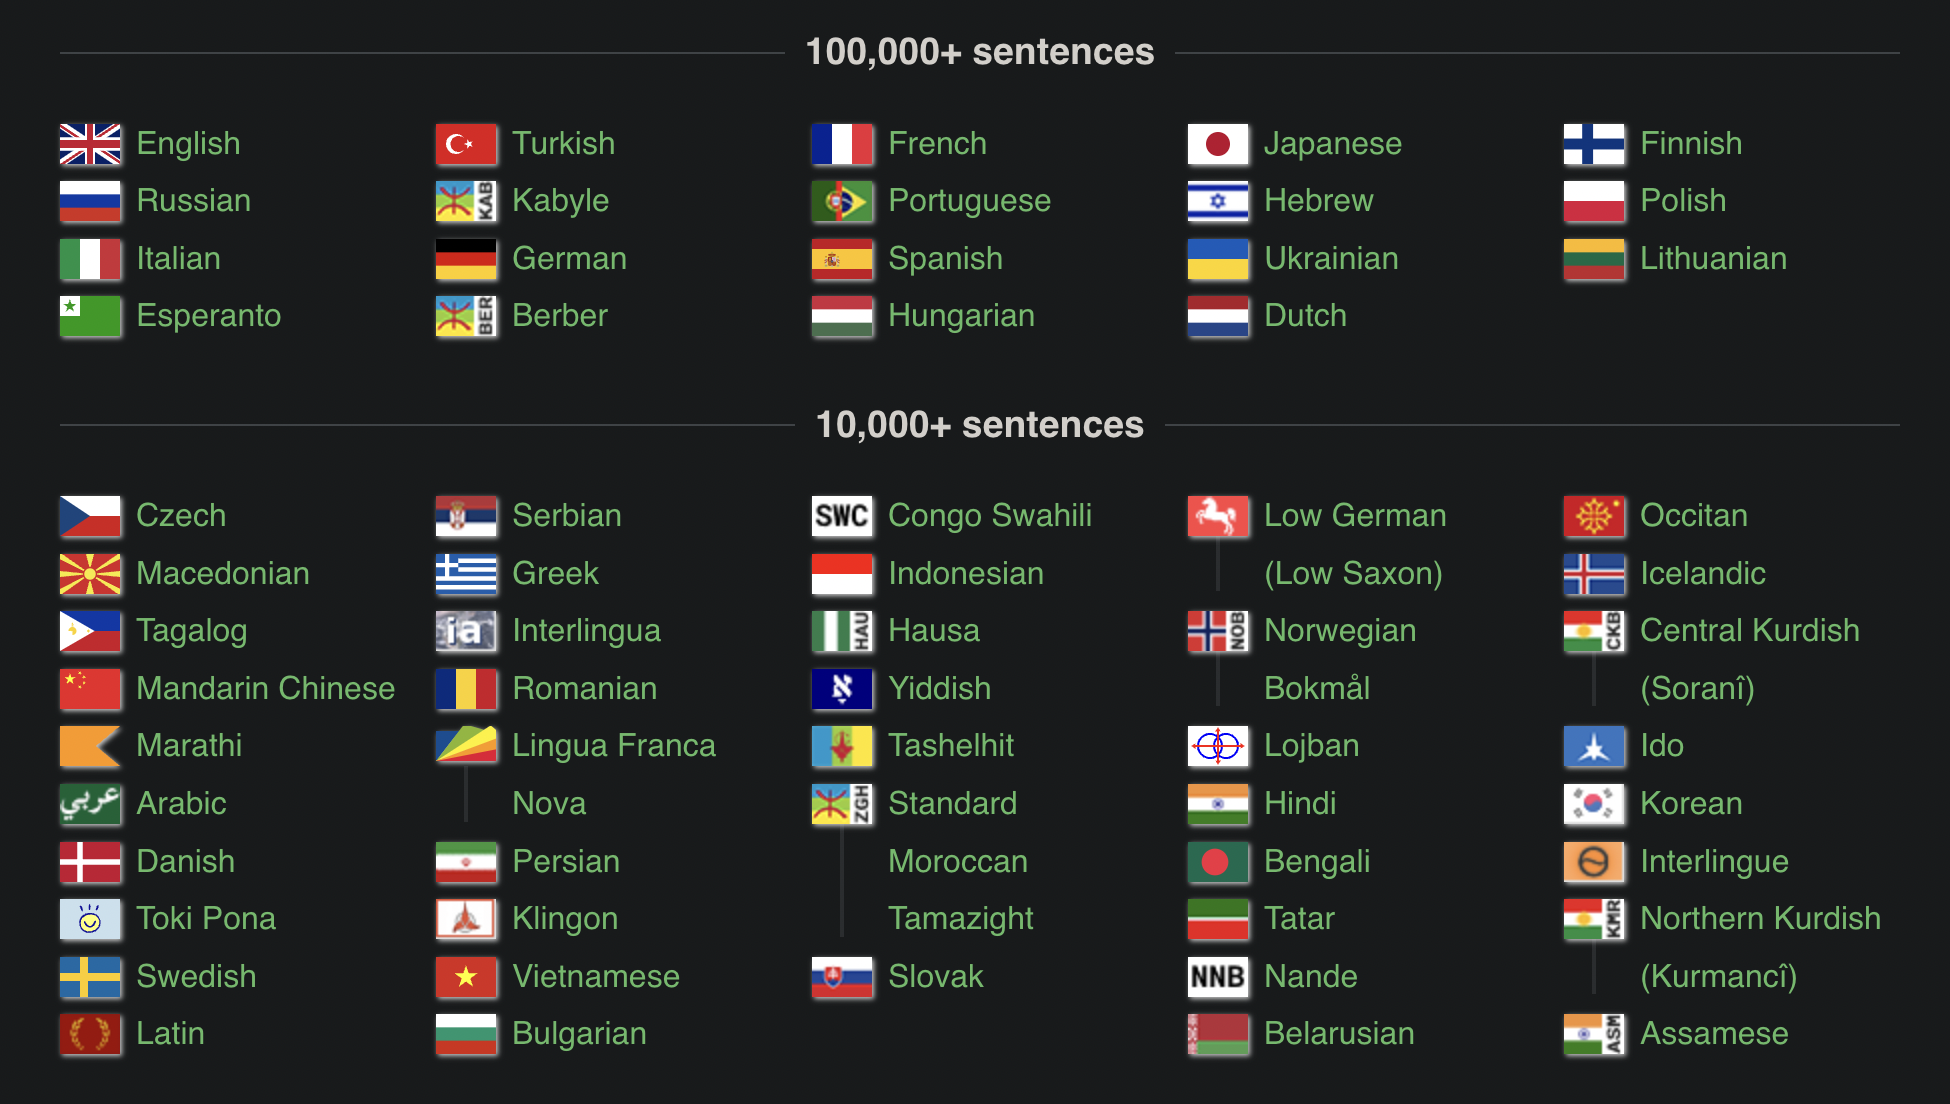
\includegraphics[width=0.9\linewidth]{images/tatoeba_languages.png}
    \caption{Tatoeba's languages repository with 10,000+ sentences and 100,000+ sentences \cite{tatoeba}}
    \label{fig:tatoeba_languages}
\end{figure}


\begin{figure}[htbp]
    \centering
    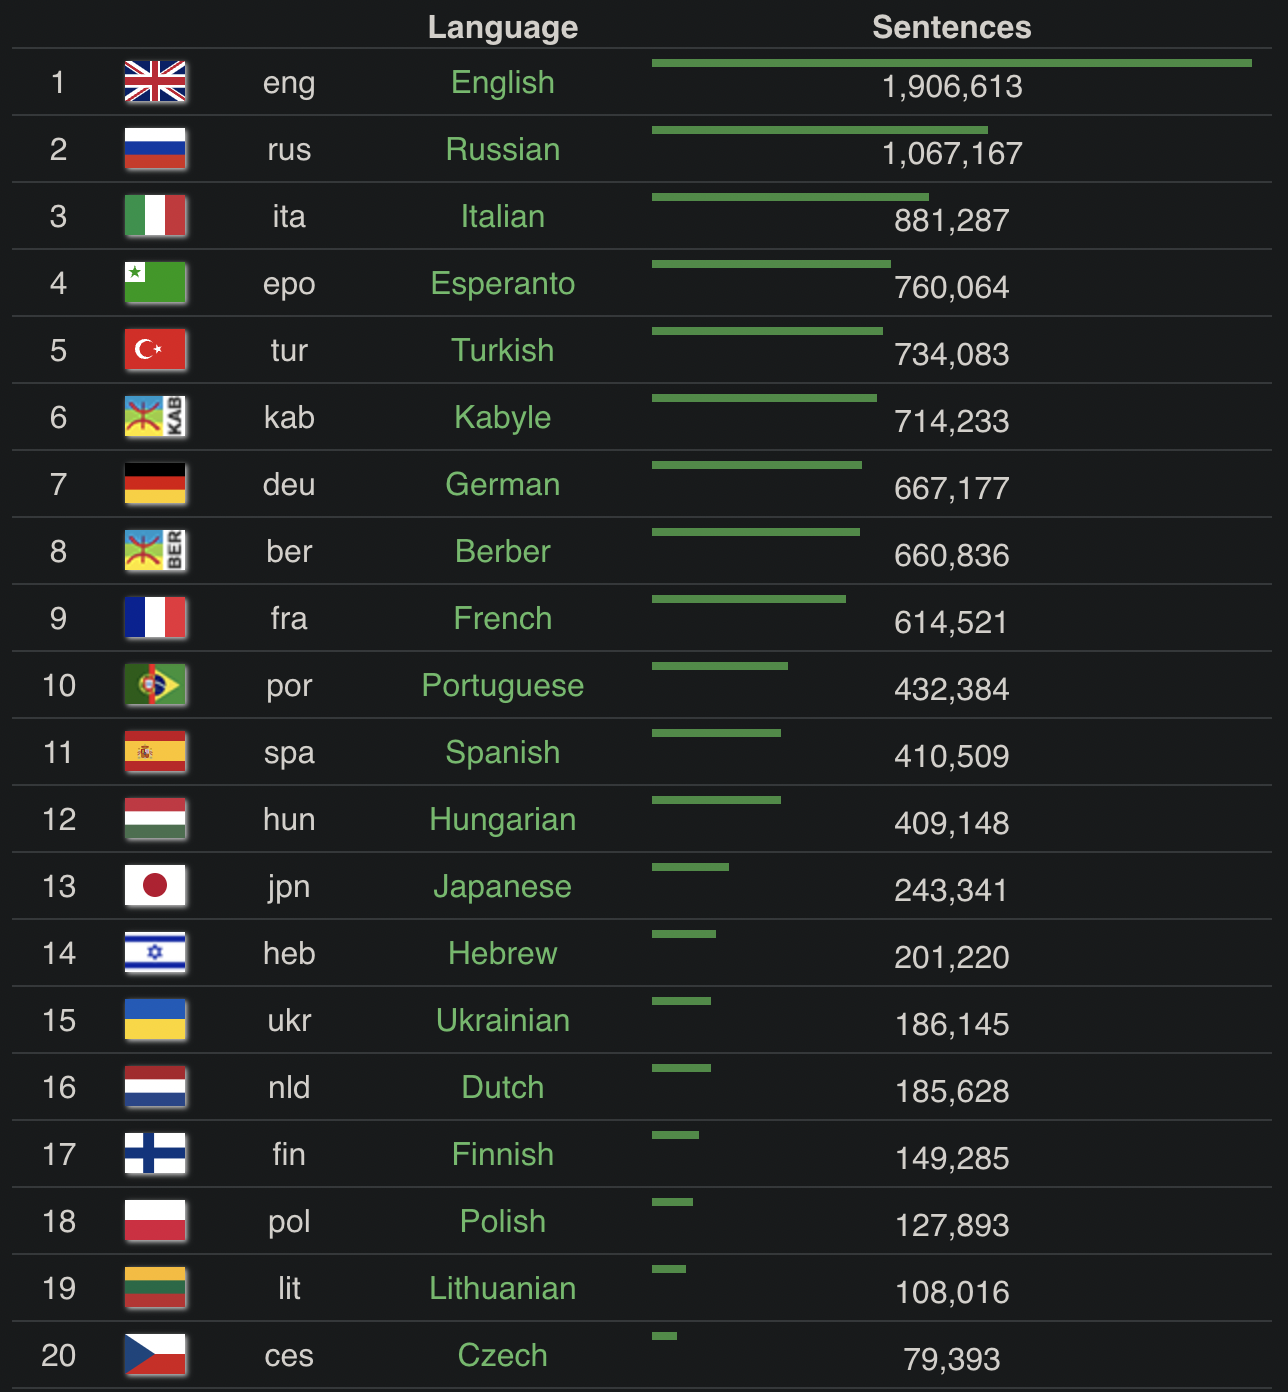
\includegraphics[width=0.5\linewidth]{images/tatoeba_top_20_lang.png}
    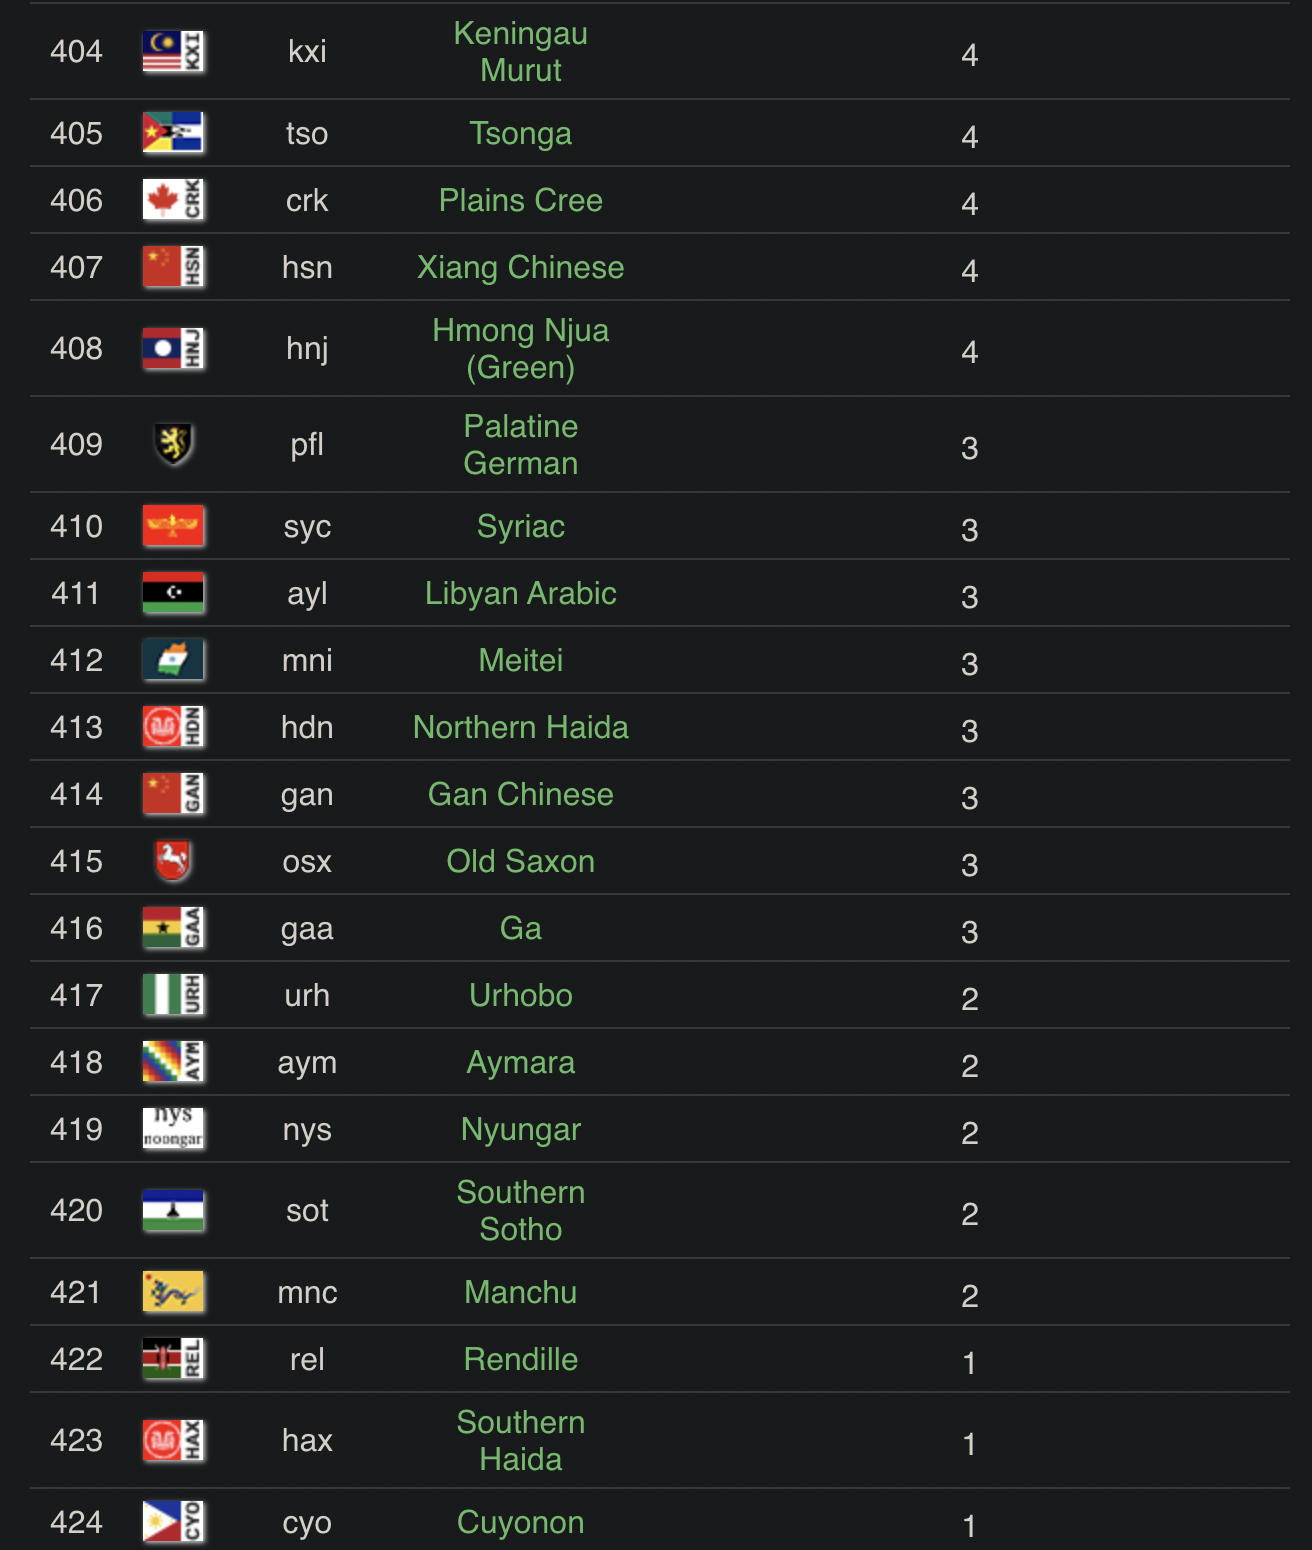
\includegraphics[width=0.46\linewidth]{images/tatoeba_bottom_20_lang.png}
    \caption{Tatoeba top 20 and bottom 20 languages based on sentences count \cite{tatoeba}}
    \label{fig:tatoeba_top_bottom_languages}
\end{figure}

\begin{table}[htbp]
    \centering
    \begin{tabular}{|l|l|}
        \hline
        \textbf{No.} & \textbf{Language} \\
        \hline
        1            & Dutch             \\
        2            & Finnish           \\
        3            & French            \\
        4            & German            \\
        5            & Hebrew            \\
        6            & Hungarian         \\
        7            & Italian           \\
        8            & Japanese          \\
        9            & Mandarin Chinese  \\
        10           & Polish            \\
        11           & Russian           \\
        12           & Spanish           \\
        13           & Turkish           \\
        14           & Ukrainian         \\
        \hline
    \end{tabular}
    \caption{List of chosen languages for evaluation}
    \label{table:eval_languages}
\end{table}

Table \ref{table:eval_languages} show the 14 languages selected for this project. Languages are chosen based on its resources' availability in Tatoeba, as well as considering supported languages in most PTMs models. To build the dataset, sentences in English are first downloaded, containing 1,898,494 sentences (it is unclear why it is less than the number stated in the Tatoeba website). Then for each language, sentence pairs between English and source languages are downloaded individually and compiled. The result is a single Dataframe containing 1241 sentences in all 14 languages, this will be treated as a test set to evaluate the models performance on each language.

Sentences typically consist of everyday phrases such as 'I have to go to sleep', 'That is intriguing', and 'Where do you live?' They may also include single-word exclamations like 'Speak!' or 'Look!' Additionally, multiple sentences such as 'You may write in any language you want. On Tatoeba, all languages are considered equal', and 'Guns don't kill people. People kill people' can be found inside the corpus. A few of them also include human names, 'Compare your answer with Tom's', 'Muiriel is 20 now'. All of the sentences are straightforward and literal, without the use of linguistic devices such as metaphors or sarcasm. Therefore, machine translation process should be straightforward on this level.


READ THIS \cite{intento-2020} (exactly what this paper should do, maybe compare results and find insights)

\section{Evaluation}

\section{Conclusion}

\printbibliography
\end{document}
